% vim: set spell spelllang=en tw=100 et sw=4 sts=4 foldmethod=marker foldmarker={{{,}}} :

\documentclass[aspectratio=169,compress,10pt]{beamer}

\usepackage{tikz}
\usepackage{xcolor}
\usepackage{complexity}
\usepackage{hyperref}
\usepackage{microtype}
\usepackage{amsmath}                   % \operatorname
\usepackage{amsfonts}                  % \mathcal
\usepackage{amssymb}                   % \nexists
\usepackage[vlined]{algorithm2e} % algorithms
\usepackage{centernot}
\usepackage{listings}
\usepackage{csquotes}
\usepackage{fancyvrb}
\usepackage{bussproofs}
\usepackage{multicol}
\usepackage{booktabs}
\usepackage{mathtools}
\usepackage{pifont}
\usepackage{marvosym}
\usepackage{cancel}
\usepackage{nicefrac}

\usefonttheme{professionalfonts}

\usetikzlibrary{shapes, arrows, shadows, calc, positioning, fit, decorations.pathreplacing,
decorations.pathmorphing, shapes.misc, tikzmark, backgrounds, trees, overlay-beamer-styles}

\tikzset{processarrow/.style={->, very thick, decorate, decoration={snake, post length=0.5mm}}}
\tikzset{brace/.style={decorate, decoration={brace}, very thick}}

\definecolor{uofguniversityblue}{rgb}{0, 0.219608, 0.396078}
\definecolor{uofgheather}{rgb}{0.356863, 0.32549, 0.490196}
\definecolor{uofgaquamarine}{rgb}{0.603922, 0.72549, 0.678431}
\definecolor{uofgslate}{rgb}{0.309804, 0.34902, 0.380392}
\definecolor{uofgrose}{rgb}{0.823529, 0.470588, 0.709804}
\definecolor{uofgmocha}{rgb}{0.709804, 0.564706, 0.47451}
\definecolor{uofgsandstone}{rgb}{0.321569, 0.278431, 0.231373}
\definecolor{uofgforest}{rgb}{0, 0.2, 0.129412}
\definecolor{uofglawn}{rgb}{0.517647, 0.741176, 0}
\definecolor{uofgcobalt}{rgb}{0, 0.615686, 0.92549}
\definecolor{uofgturquoise}{rgb}{0, 0.709804, 0.819608}
\definecolor{uofgsunshine}{rgb}{1.0, 0.862745, 0.211765}
\definecolor{uofgpumpkin}{rgb}{1.0, 0.72549, 0.282353}
\definecolor{uofgthistle}{rgb}{0.584314, 0.070588, 0.447059}
\definecolor{uofgrust}{rgb}{0.603922, 0.227451, 0.023529}
\definecolor{uofgburgundy}{rgb}{0.490196, 0.133333, 0.223529}
\definecolor{uofgpillarbox}{rgb}{0.701961, 0.047059, 0}
\definecolor{uofglavendar}{rgb}{0.356863, 0.301961, 0.580392}

% {{{ theme things
\useoutertheme[footline=authortitle]{miniframes}
\useinnertheme{rectangles}

\setbeamerfont{block title}{size={}}
\setbeamerfont{title}{size=\large,series=\bfseries}
\setbeamerfont{section title}{size=\large,series=\mdseries}
\setbeamerfont{author}{size=\normalsize,series=\mdseries}
\setbeamercolor*{structure}{fg=uofguniversityblue}
\setbeamercolor*{palette primary}{use=structure,fg=black,bg=white}
\setbeamercolor*{palette secondary}{use=structure,fg=white,bg=uofgcobalt}
\setbeamercolor*{palette tertiary}{use=structure,fg=white,bg=uofguniversityblue}
\setbeamercolor*{palette quaternary}{fg=white,bg=black}
\setbeamercolor{block body}{bg=structure!10}
\setbeamercolor{block title}{bg=structure,fg=white}
\setbeamertemplate{blocks}[rounded]
\setbeamercolor*{titlelike}{parent=palette primary}

\beamertemplatenavigationsymbolsempty

\setbeamertemplate{title page}
{
    \begin{tikzpicture}[remember picture, overlay]
        \node at (current page.north west) {
            \begin{tikzpicture}[remember picture, overlay]
                \fill [fill=uofguniversityblue, anchor=north west] (0, 0) rectangle (\paperwidth, -2.6cm);
            \end{tikzpicture}
        };

        \node (logo) [anchor=north east, shift={(-0.8cm,-0.2cm)}] at (current page.north east) {
            
\includegraphics[keepaspectratio=true,scale=0.5]{../../images/UoG_keyline.pdf}
        };

        \node (logo2) [anchor=north, below=0.2cm of logo.south] {
            
\includegraphics[keepaspectratio=true,scale=0.1]{../../images/RAEngWhite.pdf}
        };

        \coordinate (logos) at ($(logo.south)!0.5!(logo2.north)$);

        \node [anchor=west, xshift=0.8cm] at (current page.west |- logos) {
            \begin{minipage}{0.65\paperwidth}\raggedright
                {\usebeamerfont{title}\usebeamercolor[white]{}\inserttitle}\\[0.1cm]
                {\usebeamerfont{author}\usebeamercolor[white]{}\insertauthor}
            \end{minipage}
        };
    \end{tikzpicture}
}

\setbeamertemplate{section page}
{
    \begin{centering}
        \begin{beamercolorbox}[sep=12pt,center]{part title}
            \usebeamerfont{section title}\insertsection\par
        \end{beamercolorbox}
    \end{centering}
}

\newcommand{\frameofframes}{/}
\newcommand{\setframeofframes}[1]{\renewcommand{\frameofframes}{#1}}

\makeatletter
\setbeamertemplate{footline}
{%
    \begin{beamercolorbox}[colsep=1.5pt]{upper separation line foot}
    \end{beamercolorbox}
    \begin{beamercolorbox}[ht=2.5ex,dp=1.125ex,%
        leftskip=.3cm,rightskip=.3cm plus1fil]{author in head/foot}%
        \leavevmode{\usebeamerfont{author in head/foot}\insertshortauthor}%
        \hfill%
        {\usebeamerfont{institute in head/foot}\usebeamercolor[fg]{institute in head/foot}\insertshortinstitute}%
    \end{beamercolorbox}%
    \begin{beamercolorbox}[ht=2.5ex,dp=1.125ex,%
        leftskip=.3cm,rightskip=.3cm plus1fil]{title in head/foot}%
        {\usebeamerfont{title in head/foot}\insertshorttitle}%
        \hfill%
        {\usebeamerfont{frame number}\usebeamercolor[fg]{frame number}\insertframenumber~\frameofframes~\inserttotalframenumber}
    \end{beamercolorbox}%
    \begin{beamercolorbox}[colsep=1.5pt]{lower separation line foot}
    \end{beamercolorbox}
}

\makeatletter
\setbeamertemplate{mini frame}
{%
  \begin{pgfpicture}{0pt}{0pt}{.04cm}{.04cm}
    \pgfpathcircle{\pgfpoint{0.04cm}{0.04cm}}{0.04cm}
    \pgfusepath{fill,stroke}
  \end{pgfpicture}%
}
\setbeamertemplate{mini frame in current subsection}
{%
  \begin{pgfpicture}{0pt}{0pt}{.04cm}{.04cm}
    \pgfpathcircle{\pgfpoint{0.04cm}{0.04cm}}{0.04cm}
    \pgfsetfillcolor{section in head/foot.bg}
    \pgfusepath{fill,stroke}
  \end{pgfpicture}%
}

\setbeamersize{mini frame size=0.10cm, mini frame offset=0.06cm}
\makeatother

\makeatletter
\newenvironment{nearlyplainframe}[2][]{
    \def\beamer@entrycode{\vspace*{-\headheight}\vspace*{3pt}}
    \setbeamertemplate{headline}
    {%
        \begin{beamercolorbox}[colsep=1.5pt]{upper separation line head}
        \end{beamercolorbox}
        \begin{beamercolorbox}[ht=0.5ex,dp=0.125ex,%
            leftskip=.3cm,rightskip=.3cm plus1fil]{title in head/foot}%
        \end{beamercolorbox}%
        \begin{beamercolorbox}[ht=0.5ex,dp=0.125ex,%
            leftskip=.3cm,rightskip=.3cm plus1fil]{author in head/foot}%
        \end{beamercolorbox}%
        \begin{beamercolorbox}[colsep=1.5pt]{lower separation line head}
        \end{beamercolorbox}
        \vspace*{\headheight}
    }

    \setbeamertemplate{footline}
    {%
        \begin{beamercolorbox}[colsep=1.5pt]{upper separation line foot}
        \end{beamercolorbox}
        \begin{beamercolorbox}[ht=0.5ex,dp=0.125ex,%
            leftskip=.3cm,rightskip=.3cm plus1fil]{author in head/foot}%
        \end{beamercolorbox}%
        \begin{beamercolorbox}[ht=0.5ex,dp=0.125ex,%
            leftskip=.3cm,rightskip=.3cm plus1fil]{title in head/foot}%
        \end{beamercolorbox}%
        \begin{beamercolorbox}[colsep=1.5pt]{lower separation line foot}
        \end{beamercolorbox}
    }

    \begin{frame}[#1]{#2}
    }{
    \end{frame}
}
\makeatother

% }}}

\newcommand<>{\alertred}[1]{{\color#2{uofgthistle}#1}}
\renewcommand<>{\alert}[1]{{\color#2{uofgthistle}#1}}
\newcommand<>{\alertblue}[1]{{\color#2{uofgcobalt}#1}}
\newcommand<>{\alertgreen}[1]{{\color#2{uofglawn}#1}}

\author{Ciaran McCreesh}
\title{Proof Logging for Constraint Programming}

\begin{document}

{
    \usebackgroundtemplate{
        \tikz[overlay, remember picture]
        \node[at=(current page.south), anchor=south, inner sep=0pt, yshift=-1.4cm]{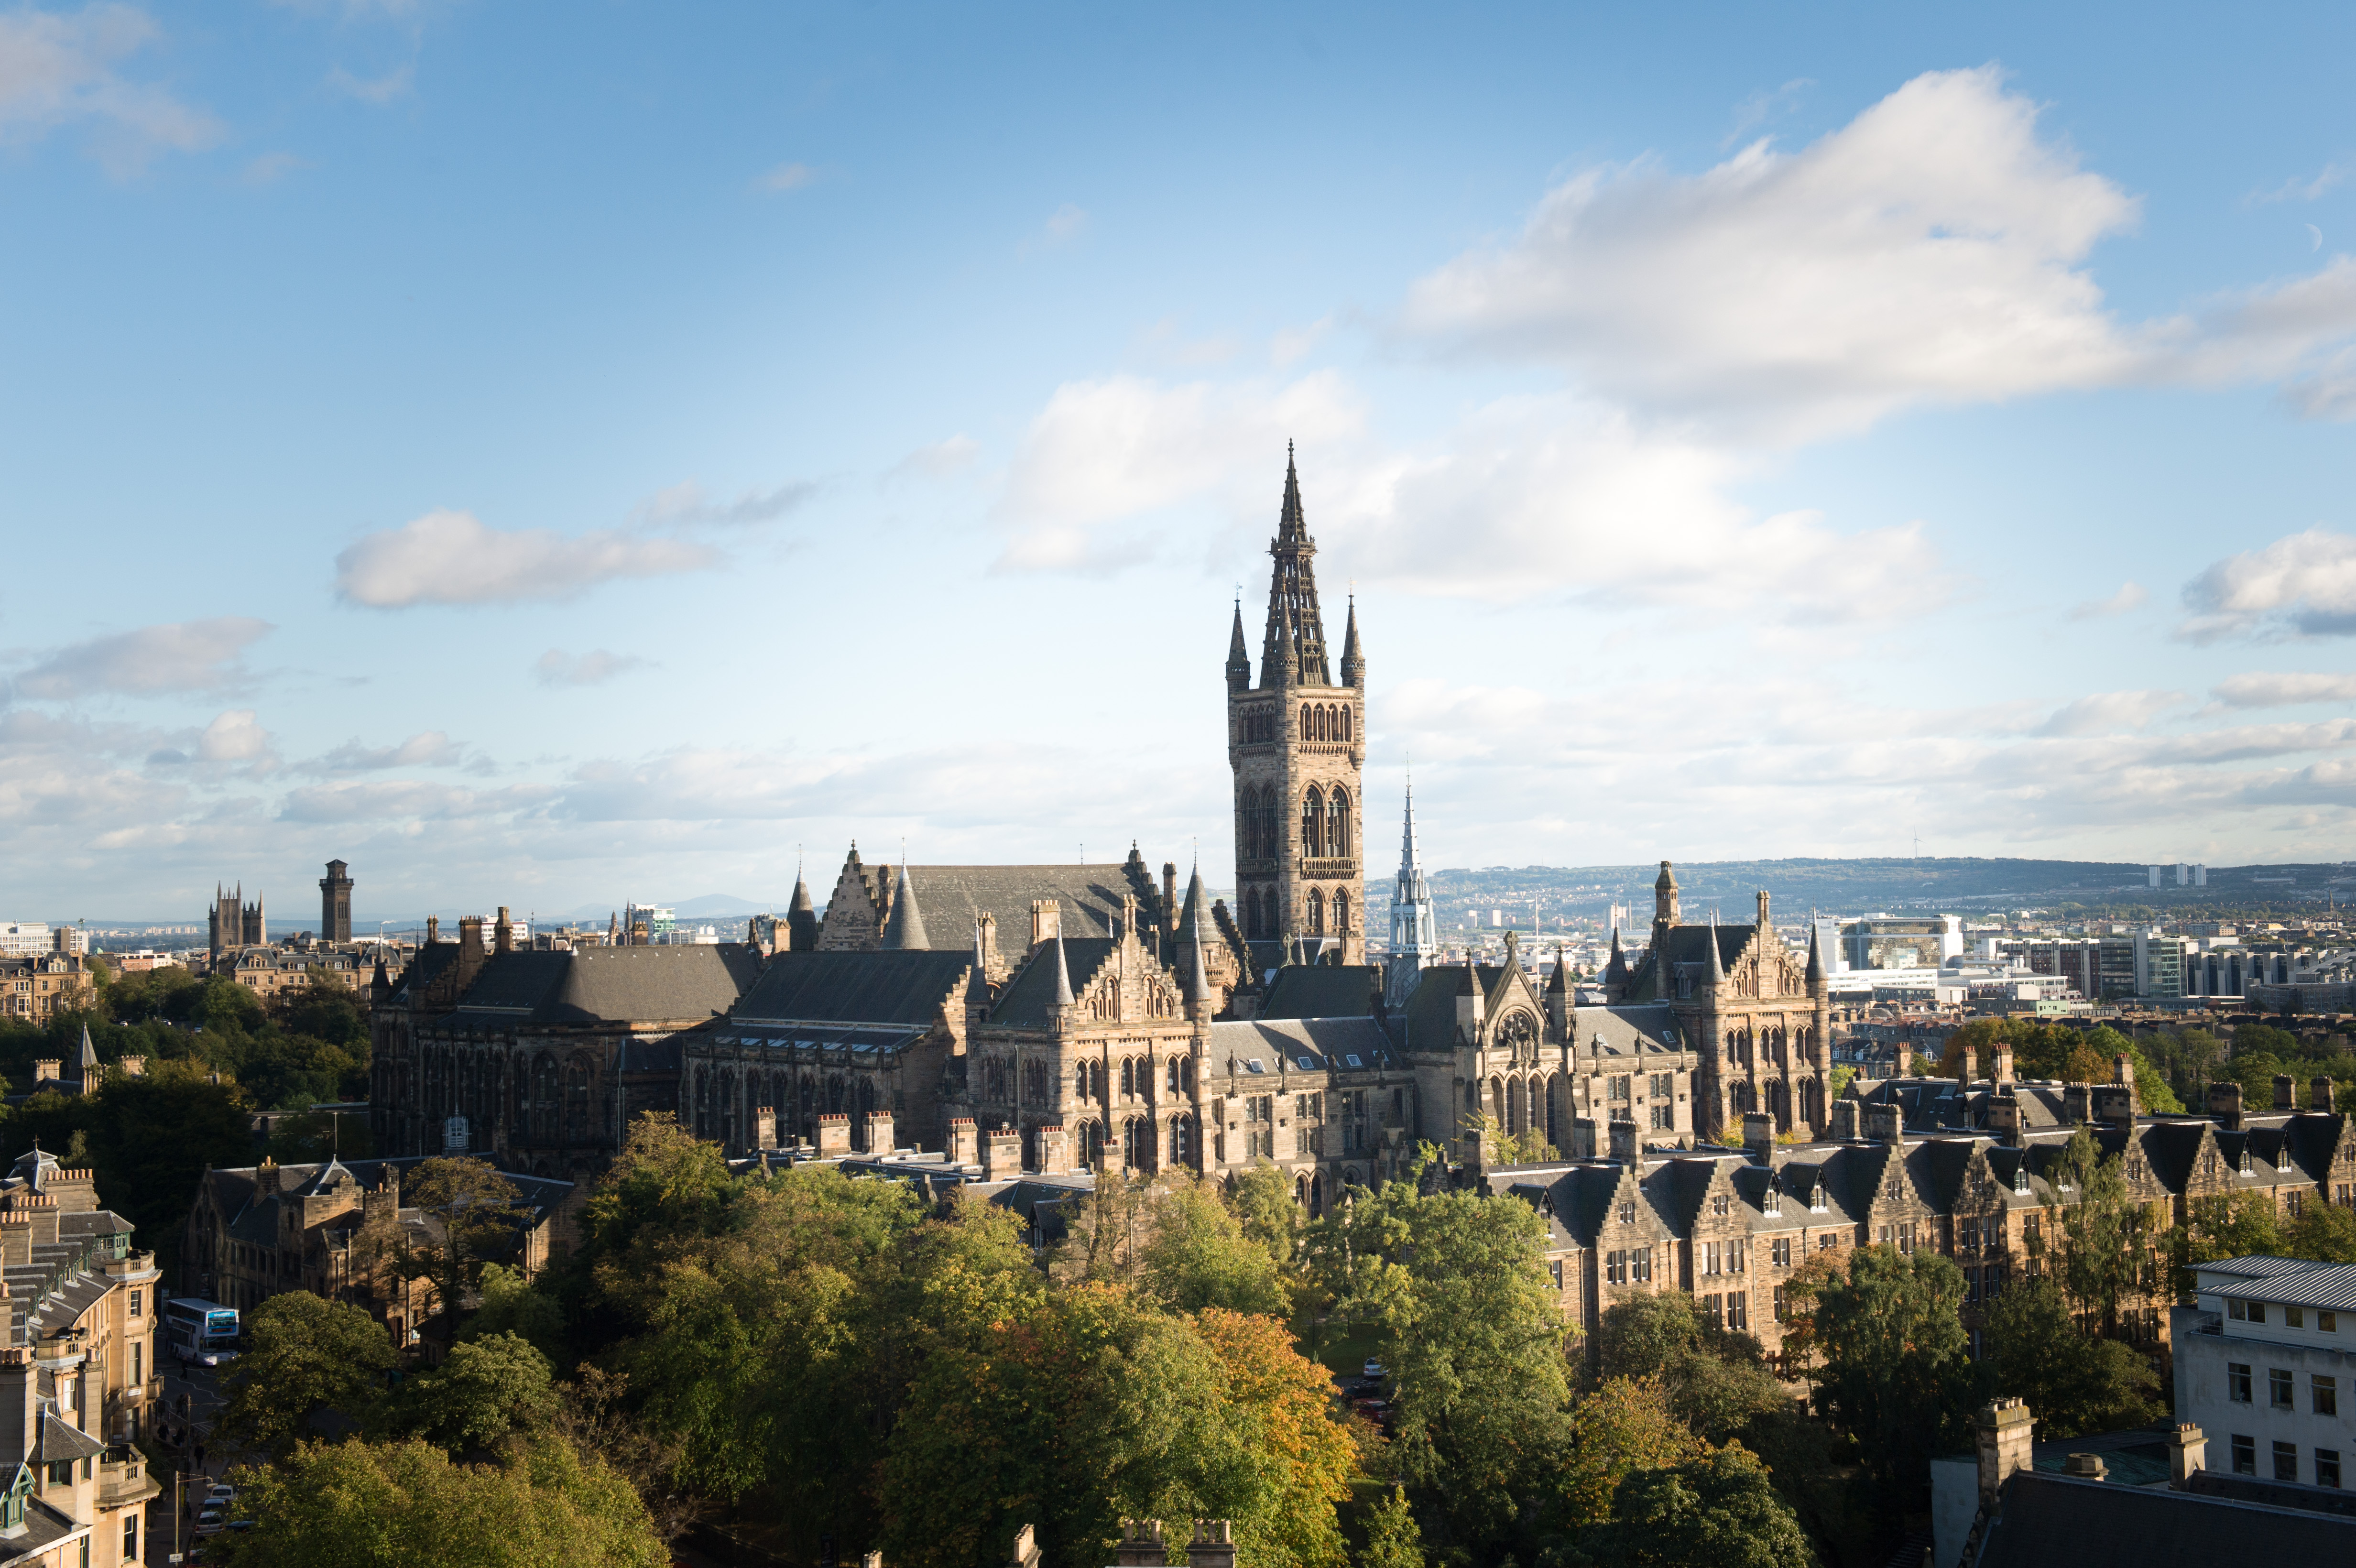
\includegraphics[keepaspectratio=true, width=\paperwidth]{../../images/background.jpg}};
    }
    \begin{frame}[plain,noframenumbering]
        \titlepage
    \end{frame}
}

\section{Proof Logging}

\begin{frame}{Proof Logging}
    \vspace*{-1.0em}
    \begin{center}
        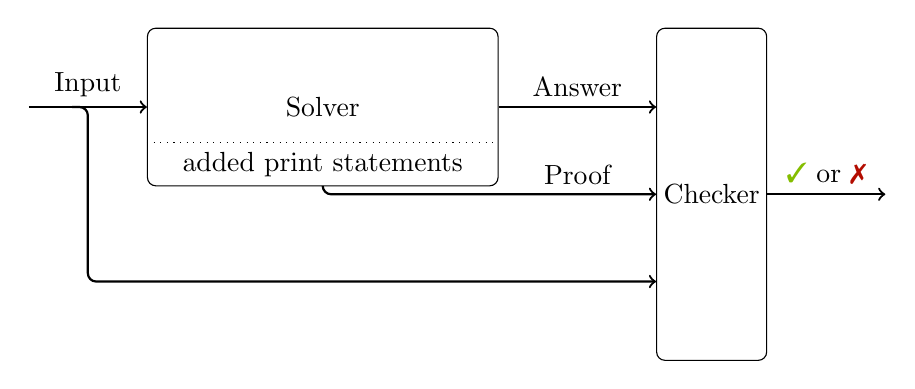
\begin{tikzpicture}
            \node (solver) [inner xsep=5em, inner ysep=2.5em, draw, rounded corners=3pt] { Solver };

            \node (checker) [right=2cm of solver.north east, anchor=north west, inner xsep=0.25em, draw, rounded corners=3pt, minimum height=12em, visible on=<3->] { Checker };

            \node (print) [anchor=south, above=0cm of solver.south, visible on=<2->] { added print statements };
            \draw [dotted, visible on=<2->] (solver.west|-print.north) -- (solver.east|-print.north);

            \draw [->, thick] (solver.east) -- (solver.east -| checker.west)
            coordinate [midway] (solutionmid) node [above, midway] { Answer };

            \draw [->, thick, rounded corners=3pt, visible on=<2->] (solver.south) -- (solver.south |- checker.west)
            -- (checker.west) coordinate [midway] (proofmid);

            \coordinate (prooflabel) at (proofmid-|solutionmid);
            \node [above=0cm of prooflabel, visible on=<2->] { Proof };

            \coordinate [right=1.5cm of checker.east] (verified);
            \draw [->, thick, visible on=<4->] (checker.east) -- (verified) node [above, midway] { \textcolor{uofglawn}{\ding{51}} or \textcolor{uofgpillarbox}{\ding{55}} };

            \coordinate [left=1.5cm of solver.west] (input);
            \draw [->, thick] (input) -- (solver.west) coordinate [midway] (inputmid) node [above, midway] { Input };

            \coordinate (checkerbotleft) at ($(checker.west)+($(checker.west)-(solver.east-|checker.west)$)$);

            \draw [->, thick, rounded corners=3pt, visible on=<3->] ($(inputmid)+(-0.2,0)$) -- (inputmid) -- (inputmid |- checkerbotleft) -- (checkerbotleft);
        \end{tikzpicture}
    \end{center}
    \vspace*{-0.7em}
    \begin{enumerate}
        \item<1->
            Run solver on problem input.
        \item<2->
            Solver also prints out a proof as part of its output.
        \item<3->
            Feed input + solution + proof to proof checker.
        \item<4->
            Verify that proof checker says solution is correct.
    \end{enumerate}
\end{frame}

\begin{frame}{The Slide That Keeps Getting Me Into Trouble}
    2021 MiniZinc challenge: for 1.28\% of instances, wrong solutions were claimed.
    \\
    \begin{itemize}
        \item False claims of unsatisfiability.
        \item False claims of optimality.
        \item Infeasible solutions produced.
        \item Not limited to a single solver, problem, or constraint.
        \item Not even consistent---same solver on same hardware and same instance can give
            different results on different runs.
    \end{itemize}
\end{frame}

\begin{frame}{How We Can Fix This}
    \begin{center}
        \begin{tikzpicture}
            \node (solver) [ inner xsep=4em, inner ysep=2.5em, draw, rounded corners=3pt] { Solver };
            \node (elaborator) [ right=2cm of solver.north east, anchor=north west, inner
            xsep=0.25em, draw, rounded corners=3pt, minimum height=12em, text width=5em, text centered] {
                \only<1>{Checker}\only<2->{Elaborator, Justifier, and Trimmer} };
            \node (verifiedchecker) [ right=2cm of elaborator.north east, anchor=north west, inner
                xsep=0.25em, draw, rounded corners=3pt, minimum height=8em, text width=4em, text
                centered, yshift=-2cm, visible on=<3->] { Verified Checker };

            \node (print) [anchor=south, above=0cm of solver.south] { added print statements };
            \draw [dotted] (solver.west|-print.north) -- (solver.east|-print.north);

            \draw [->, thick] (solver.east) -- (solver.east -| elaborator.west) coordinate [midway]
            (solutionmid) node [above, midway] { Answer };

            \draw [->, thick, rounded corners=3pt] (solver.south) -- (solver.south |- elaborator.west) -- (elaborator.west) coordinate [midway] (proofmid);

            \coordinate (prooflabel) at (proofmid-|solutionmid); \node [above=0cm of prooflabel] { Proof };

            \coordinate [right=2cm of verifiedchecker.east] (verified);
            \draw [->, thick, visible on=<3>] (verifiedchecker.east) -- (verified)
                node [above, midway] { \textcolor{uofglawn}{\ding{51}} or \textcolor{uofgpillarbox}{\ding{55}} }
                node [below, midway, text centered, text width=5em] { Trusted Answer };
            \draw [->, thick, visible on=<4>] (verifiedchecker.east) -- (verified)
                node [above, midway] { \textcolor{uofglawn}{\ding{51}} or \textcolor{uofgpillarbox}{\ding{55}} }
                node [below, midway, text centered, text width=5em] { Trusted Answer in Domain Language };

            \coordinate [left=1.5cm of solver.west] (input);
            \draw [->, thick] (input) -- (solver.west) coordinate [midway] (inputmid) node [above, midway] { Input };

            \coordinate (verifiedcheckertopleft) at ($(verifiedchecker.west)+($(0cm,1.2cm)$)$);
            \draw [->, thick, visible on=<2->] (elaborator.east |- verifiedcheckertopleft) --
            (verifiedcheckertopleft) node [above, midway, text width=4em, text centered] { Answer };
            \draw [->, thick, visible on=<2->] (elaborator.east |- verifiedchecker.west) -- (verifiedchecker.west) node [above, midway, text width=4em, text centered] { Kernel Proof };

            \coordinate (elaboratorbotleft) at ($(elaborator.west)+($(elaborator.west)-(solver.east-|elaborator.west)$)$);
            \coordinate (verifiedcheckerbotleft) at ($(verifiedchecker.west)+($(0cm,-1.2cm)$)$);

            \coordinate (elaboratortopright) at ($(elaborator.east)+($(verifiedcheckertopleft)-(verifiedchecker.west)$)$);
            \draw [->, thick] (elaboratortopright) -- (elaboratortopright-|verifiedchecker.west)
                node [above, midway] { \textcolor{uofglawn}{\ding{51}} or \textcolor{uofgpillarbox}{\ding{55}} };

            \coordinate (solverstart) at ($(solver.south)!0.75!(solver.south west)$);
            \coordinate (checkerbotleft) at ($(elaborator.west)+($(elaborator.west)-(solver.east-|elaborator.west)$)$);
            \draw [->, thick, rounded corners=3pt] (solverstart) -- (solverstart |- checkerbotleft) -- (checkerbotleft)
            coordinate [midway] (altinputmid);

            \coordinate (encinputlabel) at (altinputmid-|solutionmid);
            \node [above=0cm of encinputlabel, xshift=-0.5cm] { Encoded Input };

            \draw [->, thick, rounded corners=3pt, visible on=<3>] (solverstart) -- (solverstart |- verifiedcheckerbotleft) -- (verifiedcheckerbotleft);
            \draw [->, thick, rounded corners=3pt, visible on=<4>] ($(inputmid)+(-0.2,0)$) --
            (inputmid) -- (inputmid |- verifiedcheckerbotleft) -- (verifiedcheckerbotleft)
            coordinate [midway] (verinputmid);

            \coordinate (verinputlabel) at (verinputmid-|solutionmid);
            \node [above=0cm of verinputlabel, xshift=-0.5cm, visible on=<4>] { Verified Input };
        \end{tikzpicture}
    \end{center}
\end{frame}

\begin{frame}{The Ludicrous Hypothesis}
    \begin{block}{}
        A constraint programming solver can justify \alertred{everything} it does, in a proof format
        that knows \alertred{nothing} about constraint programming.
    \end{block}

    Four reasons this cannot possibly work:
    \begin{itemize}
        \item<2->
            \alertblue{Can it say it?} The format has 0/1 variables and linear inequalities over
            them. We have integer variables, and a catalogue of several hundred global constraints.

        \item<3->
            \alertblue{Can it prove it?} Existing is not enough, proofs have to be short. The system
            SAT solvers reason in needs exponentially many steps to refute the pigeonhole principle.

        \item<4->
            \alertblue{Can we work it out?} A propagator is an algorithm rather than a deduction:
            matching, flow, dynamic programming, automata. Someone has to find the argument it is
            making.

        \item<5->
            \alertblue{Can we afford it?} Nobody leaves proof logging on if it costs a hundred times
            as much, or if the proof is too big to check.
    \end{itemize}

    \smallskip

    \uncover<6->{It mostly works. One format, one checker, and adding a constraint to your solver
    adds nothing to what you have to trust.}
\end{frame}

\section{Encoding CP Variables}

\begin{frame}{The Direct Encoding}
    An encoding has to \alertblue{mean} what the variable means, and it has to provide every atom a
    propagator might want to talk about. It does \alertred{not} have to propagate well: nobody is
    solving this, we are only checking it.

    \medskip

    Upper case $X$ for a constraint programming variable, lower case for pseudo-Boolean atoms. For
    $X \in \{0 \ldots 7\}$, one atom per value, with $x_{=v}$ meaning $X = v$:
    \begin{equation*}
        x_{=0} + x_{=1} + x_{=2} + x_{=3} + x_{=4} + x_{=5} + x_{=6} + x_{=7} = 1
    \end{equation*}

    \begin{itemize}
        \item<2->[\textcolor{uofglawn}{\ding{51}}]
            This is what a solver thinks a variable is. A domain is a set of atoms, and deleting a
            value is falsifying one.
        \item<3->[\textcolor{uofgpillarbox}{\ding{55}}]
            One atom per value. A variable over $\{0 \ldots 10^6\}$ is a million atoms before anyone
            has written a constraint.
        \item<4->[\textcolor{uofgpillarbox}{\ding{55}}]
            Arithmetic is clumsy. $X$ itself is $\sum_v v \cdot x_{=v}$, so adding up three
            variables needs a term for every value of every one of them.
    \end{itemize}
\end{frame}

\begin{frame}{The Order Encoding}
    One atom per value again, but $x_{\ge v}$ meaning $X \ge v$. Nothing says so yet, so we say it:
    \begin{equation*}
        x_{\ge 2} \Rightarrow x_{\ge 1}, \qquad x_{\ge 3} \Rightarrow x_{\ge 2}, \qquad \ldots
        \qquad x_{\ge 7} \Rightarrow x_{\ge 6}
    \end{equation*}
    each of which is the pseudo-Boolean constraint $x_{\ge v} + \overline{x_{\ge v + 1}} \ge 1$.

    \medskip

    \begin{itemize}
        \item<2->[\textcolor{uofglawn}{\ding{51}}]
            A bound is one literal. Most propagators reason about bounds, and now they have
            something to reason with.
        \item<3->[\textcolor{uofglawn}{\ding{51}}]
            The direct atoms come back for free, since $X = v$ is a bound from each side:
            \begin{equation*}
                x_{=v} \Leftrightarrow x_{\ge v} \wedge \overline{x_{\ge v + 1}}
            \end{equation*}
        \item<4->[\textcolor{uofgpillarbox}{\ding{55}}]
            Still one atom per value, and arithmetic is still clumsy.
    \end{itemize}
\end{frame}

\begin{frame}{The Bits Encoding}
    Say what the variable \alertblue{is}, in binary, and introduce no atoms for values at all:
    \begin{equation*}
        X = 1 x_{\operatorname{b}0} + 2 x_{\operatorname{b}1} + 4 x_{\operatorname{b}2}
    \end{equation*}
    with one extra constraint bounding $X$ from above, when the domain is not a power of two long.

    \medskip

    \begin{itemize}
        \item<2->[\textcolor{uofglawn}{\ding{51}}]
            Logarithmic. A million values is twenty atoms.
        \item<3->[\textcolor{uofglawn}{\ding{51}}]
            Arithmetic is free. $X + Y - Z \le 4$ \emph{is} a pseudo-Boolean constraint once the
            bits are substituted in: one row, not one row per value.
        \item<4->[\textcolor{uofgpillarbox}{\ding{55}}]
            There is nothing to say. No atom means $X \ge 4$, or $X \ne 3$, and those are exactly
            what a propagator infers.
    \end{itemize}

    \medskip

    \uncover<5->{\small Negative domains want a sign bit, with coefficient $-2^n$. Kindling has
    none: every domain starts at zero, which keeps every coefficient positive and every atom name
    free of a minus sign.}
\end{frame}

\begin{frame}{Hybrid Encodings}
    Have all three, and say how they relate:
    \begin{align*}
        x_{\ge v} &\Leftrightarrow 1 x_{\operatorname{b}0} + 2 x_{\operatorname{b}1}
        + 4 x_{\operatorname{b}2} \ge v \\
        x_{=v} &\Leftrightarrow x_{\ge v} \wedge \overline{x_{\ge v + 1}}
    \end{align*}

    \begin{itemize}
        \item<2->
            The \alertblue{bits} say what the variable is, and carry every linear constraint.
        \item<3->
            The \alertblue{order} atoms are the currency of inference: whatever a propagator learns,
            it learns as one of these.
        \item<4->
            The \alertblue{direct} atoms are what table and all-different are made of. Defined from
            the order atoms rather than from the bits, which will matter later.
        \item<5->
            Each of these is a \alertred{definition}. It says nothing about the problem, only about
            what the atoms mean, so it is always available and always true.
    \end{itemize}

    \medskip

    \uncover<6->{Moving between the layers is what most of a proof will turn out to be doing.}
\end{frame}

\begin{frame}{Kindling: a Vibe-Coded Solver, with Proof Logging}
    Under two thousand lines of Python, with no dependencies. Non-negative bounded integer
    variables, three constraints, depth-first search by cloning, no learning, and unsatisfiable
    instances only. It writes an \texttt{.opb} saying what the problem means and a \texttt{.pbp}
    saying what it did. It is deliberately unpolished: it exists to be taken apart.

    \begin{itemize}
        \item<2->
            The encoding is the one two slides ago, written out in full for every variable before
            the search starts. With three constraints, every atom anyone will ever mention is known
            in advance.
        \item<3->
            It was written entirely by Claude --- design, proofs, tests --- and it steals heavily
            from the Glasgow Constraint Solver. It found two bugs in VeriPB on the way.
        \item<4->
            The usual objection to proof logging is the effort: someone has to work out the argument
            for each of hundreds of propagators. That objection is getting much weaker.
        \item<5->
            You should not trust a solver because of who wrote it. That is the whole point, and it
            applies to this one too.
    \end{itemize}
\end{frame}

\begin{frame}{Doing This Lazily}
    Writing every atom out in advance does not scale. One variable over $\{0 \ldots 10^6\}$ is a
    couple of million rows in the model before anything has been solved, and nearly every one of
    those atoms will never be mentioned again.

    \medskip

    \begin{itemize}
        \item<2->
            So do not write them. Keep the \alertblue{bits} in the model, and introduce $x_{\ge v}$
            the first time a propagator wants to say something about $v$ --- in the \alertred{proof}
            rather than in the model.
        \item<3->
            This is sound because these rows are \alertred{definitions}. They say what a brand new
            atom means and nothing about anything else, so they cannot turn an unsatisfiable problem
            into a satisfiable one. Checkers have a rule for exactly this: in VeriPB it is
            \texttt{red}.
        \item<4->
            Each new atom is also linked to the neighbours it turns out to have, handing the checker
            $x_{\ge v} \Rightarrow x_{\ge j}$ for the closest $j < v$ that exists. At the top of the
            proof, never in the model.
        \item<5->
            Those links are not assumptions either. They follow from the definitions, and one
            cutting planes line derives each --- once, rather than every time the checker wants it.
    \end{itemize}
\end{frame}

\begin{frame}{The Glasgow Constraint Solver}
    The real one, and the solver kindling is a small copy of. C++, around forty constraints, and
    every inference every one of them makes is justified.

    \medskip

    \begin{itemize}
        \item<2->
            Bits in the model, order and direct atoms introduced lazily in the proof, exactly as on
            the previous slide.
        \item<3->
            All-different by Hall sets, table, regular, element, circuit, cumulative with
            time-tabling and edge finding, knapsack by dynamic programming, and so on. Several of
            these took a paper each.
        \item<4->
            Optimisation as well as satisfaction, so the proof has to justify the bounds too, and
            not only the failures.
        \item<5->
            Everything in the rest of this talk is in there, in a version that also has to be fast.
    \end{itemize}

    \medskip

    \uncover<6->{\small\url{https://github.com/ciaranm/glasgow-constraint-solver}}
\end{frame}

\begin{frame}{Properties of This Encoding}
    All this effort goes on integer variables, so that propagators and search become easy to write.

    \begin{itemize}
        \item<2->
            \alertblue{It stays small.} A \texttt{var int} in MiniZinc has astronomical bounds:
            sixty-odd bits, plus an atom for each value anyone mentioned. A direct or an order
            encoding would not survive the declaration.

        \item<3->
            \alertblue{The layers stay in step.} Anything said in one is mirrored into the others by
            unit propagation alone: fix some bits and the order and direct atoms follow; assert an
            order atom and the bits follow, and so does everything that bound implies.

        \item<4->
            So a propagator says what it means in whichever layer suits it, and nothing has to be
            maintained: the order chain is already unit propagation, and ``takes at least one
            value'' is a line of cutting planes rather than an axiom --- the lines at the top of
            every kindling proof.

        \item<5->
            This is a \alertred{pseudo-Boolean} property, not a Boolean one. One constraint compares
            a bit vector against a number, and propagates the moment a coefficient exceeds the
            slack. No clause does that, and encoding the comparison in clauses loses it --- a real
            cost for solvers that live in CNF.
    \end{itemize}

    \uncover<6->{\small Stated properly as Theorem 3.3 and friends, in Matthew McIlree's thesis.}
\end{frame}

\section{Encoding CP Constraints}

\begin{frame}{Linear Inequalities}
    Substitute the bits, and there is nothing left to do. For $X, Y, Z \in \{0 \ldots 7\}$, the
    constraint $2X + 3Y - Z \le 12$ is
    \begin{align*}
        2x_{\operatorname{b}0} + 4x_{\operatorname{b}1} + 8x_{\operatorname{b}2}
        + 3y_{\operatorname{b}0} + 6y_{\operatorname{b}1} + 12y_{\operatorname{b}2}
        - z_{\operatorname{b}0} - 2z_{\operatorname{b}1} - 4z_{\operatorname{b}2} \le 12
    \end{align*}

    \begin{itemize}
        \item<2->
            One row, whatever the coefficients are, and its size depends upon how many variables
            there are rather than upon how big their domains are.
        \item<3->
            It propagates almost nothing, which is still fine.
        \item<4->
            Kindling refuses any coefficient but $\pm 1$. Not because the encoding minds, but
            because unit coefficients make every row of the \alertblue{justification} enter with
            multiplier one. Putting the coefficient back is one more operation --- and one of the
            exercises.
    \end{itemize}
\end{frame}

\begin{frame}{Reification}
    Flattening a model produces reified constraints everywhere, and an encoding wants Booleans of
    its own as well. Both are the same thing:
    \begin{equation*}
        b \Rightarrow \sum_i c_i x_i \ge d
        \qquad\text{becomes}\qquad
        \sum_i c_i x_i + M \overline{b} \ge d
    \end{equation*}
    for an $M$ big enough that the row says nothing at all when $b$ is false.

    \begin{itemize}
        \item<2->
            We have done this already. The rows tying $x_{\ge v}$ to the bits are exactly this
            shape, which is where their suspicious looking coefficients came from.
        \item<3->
            VeriPB writes it for you: \texttt{b ==> \ldots} and \texttt{b <== \ldots} normalise to
            precisely that row.
        \item<4->
            \alertred{Reify both directions.} A flag that implies its meaning, without the converse,
            never becomes true by unit propagation --- and then everything downstream that needed it
            to be true quietly stops being reverse unit propagation. This is the most common way to
            get an encoding subtly wrong.
    \end{itemize}
\end{frame}

\begin{frame}{Table Constraints}
    One Boolean per tuple, saying that this is the tuple in use. For
    $(X, Y, Z) \in [(1, 2, 3), (1, 3, 4), (2, 2, 5)]$:
    \begin{equation*}
        t_1 + t_2 + t_3 \ge 1
    \end{equation*}
    \vspace*{-1.5em}
    \begin{equation*}
        t_1 \Rightarrow x_{=1} \wedge y_{=2} \wedge z_{=3}
        \quad
        t_2 \Rightarrow x_{=1} \wedge y_{=3} \wedge z_{=4}
        \quad
        t_3 \Rightarrow x_{=2} \wedge y_{=2} \wedge z_{=5}
    \end{equation*}

    \begin{itemize}
        \item<2->
            This is what the direct atoms are for.
        \item<3->
            Deleting an unsupported value is now \alertblue{reverse unit propagation} and nothing
            else. Suppose the value is still there: the selectors fall over one at a time, until the
            row saying some tuple is in use has nothing left to satisfy it.
        \item<4->
            The tuple Booleans are proof-only. The solver never branches on them and never looks at
            them. They exist so that the argument can be written down.
    \end{itemize}
\end{frame}

\begin{frame}{All-Different (Kindling Version)}
    One at-most-one row per \alertblue{value}, over the direct atoms:
    \begin{equation*}
        \text{for each value } v: \qquad x_{1=v} + x_{2=v} + \cdots + x_{n=v} \le 1
    \end{equation*}

    \begin{itemize}
        \item<2->
            Every value gets a row, including the ones only one variable could ever take. Such a row
            says nothing by itself, but the argument we are heading for adds up the rows for a whole
            set of values, and a missing one leaves the sum short.
        \item<3->
            The size is the number of variables times the size of the domain, which is precisely
            what the last section was about avoiding.
        \item<4->
            It is here anyway, because it makes the interesting argument --- these variables will
            not fit into the values left to them --- a plain sum of rows you can read off the model.
            In a teaching solver that is worth more than being small.
    \end{itemize}
\end{frame}

\begin{frame}{All-Different (Glasgow Version)}
    A clique of not-equals instead. One flag per pair, saying which way round that pair goes, and
    two half-reified rows over the \alertblue{bits}:
    \begin{align*}
        s_{ij} &\Rightarrow X_j - X_i \le -1 \\
        \overline{s_{ij}} &\Rightarrow X_i - X_j \le -1
    \end{align*}

    \begin{itemize}
        \item<2->
            $\binom{n}{2}$ pairs, two rows each, and not one mention of a value anywhere. This does
            not grow with the domain, so an all-different over unbounded integers costs no more than
            one over $\{1 \ldots n\}$.
        \item<3->
            But the at-most-one rows the argument needs have gone. They are \alertred{consequences}
            of this encoding rather than part of it.
        \item<4->
            So derive them: in the proof, once, the first time a propagator needs one. How is the
            best example in this talk, and it is in the next section.
    \end{itemize}
\end{frame}

\section{Proofs}

\begin{frame}[fragile]{Backtracking Search}
    Two variables that a table says must agree and an all-different says must differ. Here is the
    entire proof of the search:

    \begin{Verbatim}[fontsize=\small]
@atleast1 pol @x1eq0_dn @x1eq1_dn + ;
@atleast2 pol @x2eq0_dn @x2eq1_dn + ;
% decide x1 = 0
rup 1 ~x1eq0 >= 1 ;
% decide x1 != 0
rup 1 x1eq0 >= 1 ;
rup >= 1 ;
    \end{Verbatim}

    \begin{itemize}
        \item<2->
            A guess needs no justification. Only a dead end does, and it is one line: these
            decisions cannot all hold.
        \item<3->
            The last dead end is the root, whose decision list is empty, so the line that closes the
            proof is the same line as all the others with nothing left in it.
        \item<4->
            Notice what is missing: not one word from any propagator. VeriPB accepts it anyway ---
            it redid the propagation itself.
    \end{itemize}
\end{frame}

\begin{frame}[fragile]{Propagations Aren't RUP}
    The same trick on $a + b + c \le 9$, where something else has already established $a \ge 4$,
    $b \ge 3$ and $c \ge 3$. No search is needed here at all: the propagators refute it outright.

    \begin{Verbatim}[fontsize=\small]
@atleast1 pol ... ;    @atleast2 pol ... ;    @atleast3 pol ... ;
rup >= 1 ;
    \end{Verbatim}

    \begin{itemize}
        \item<2->
            \texttt{REJECTED}, and quite right too. Nothing in that file says why the problem has no
            solution.
        \item<3->
            The solver knew perfectly well. It added the three bounds up, got $10$, and compared it
            against $9$. It simply never wrote that down --- and unlike last time, the checker
            cannot work it out for itself.
        \item<4->
            This is the load bearing fact of the whole module. Everything from here on is about what
            goes in that gap.
    \end{itemize}
\end{frame}

\begin{frame}[fragile]{Debugging a Failed Proof}
    \begin{Verbatim}[fontsize=\small,commandchars=\\\{\}]
$ veripb --trace-failed tight-sum.opb tight-sum.pbp
Propagation check failed! The propagation had the following trail:
    \alertblue{x1b2}   (4 x1b2 2 x1b1 1 x1b0 >= 4)
    \alertblue{x1ge4}  (4 ~x1b2 2 ~x1b1 1 ~x1b0 4 x1ge4 >= 4)
    \alertblue{x1ge3}  (4 ~x1b2 2 ~x1b1 1 ~x1b0 5 x1ge3 >= 5)
    \alertblue{x1ge2}  (4 ~x1b2 2 ~x1b1 1 ~x1b0 6 x1ge2 >= 6)
    \alertblue{~x1eq3} (1 ~x1ge4 1 ~x1eq3 >= 1)                 \alertred{... and then it stops}
Error: Checking error at tight-sum.pbp:8
    \end{Verbatim}

    \begin{itemize}
        \item<2->
            Every single thing the checker managed to work out is about $a$, and not one of them is
            about $b$ or $c$.
        \item<3->
            $a \ge 4$ forces the top bit, because $4$ is a power of two --- and from that one bit,
            every other atom of $a$ follows. $b \ge 3$ forces no bit at all: that row has slack
            $4$, and no coefficient bigger than it.
        \item<4->
            So $a + b + c \le 9$ never hears about $b$ or $c$. A bound and a constraint row are in
            different coordinate systems, and only cutting planes moves between them.
    \end{itemize}
\end{frame}

\begin{frame}[fragile]{Assertions for Propagations}
    The cheat: \texttt{a} adds a constraint without checking it.

    \begin{Verbatim}[fontsize=\small,commandchars=\\\{\}]
\alertred{a} 1 x2ge3 >= 1 : : int_lin_le_negative_coefficient ;
\alertred{a} 1 x3ge3 >= 1 : : int_lin_le_negative_coefficient ;
\alertred{a} 1 x1ge4 >= 1 : : int_lin_le_negative_coefficient ;
pol @lin1 @x1ge4_up + @x2ge3_up + @x3ge3_up + s ;
rup >= 1 ;

veripb: UNDER ASSERTIONS -- everything checked except what we asserted
    \end{Verbatim}

    \begin{itemize}
        \item<2->
            \texttt{UNDER ASSERTIONS} rather than \texttt{VERIFIED}, and that difference is the
            whole development process: get the scaffolding right, assert every propagator, then burn
            the assertions down one at a time. Here two of the three exercises are already done.
        \item<3->
            The annotations are meant for tools rather than for people, so the solver can tell you
            what is left to do.
        \item<4->
            \texttt{REJECTED} means something is \alertred{wrong}. \texttt{UNDER ASSERTIONS} means
            something is \alertblue{missing}. You will meet both, and they are very different days.
    \end{itemize}
\end{frame}

\section{Propagation}

\begin{frame}[fragile]{Justifying Table Constraint Inferences}
    A value with no supporting tuple left. The propagator found that with an algorithm; the proof
    says it in one line, and there is nothing to derive:

    \begin{Verbatim}[fontsize=\small]
% decide x1 = 0
rup 1 ~x1eq0 1 ~x2eq1 >= 1 ;
    \end{Verbatim}

    \begin{itemize}
        \item<2->
            Read it as an implication: if $X_1 = 0$ then $X_2 \ne 1$.
        \item<3->
            The checker assumes the opposite of that, so both $X_1 = 0$ and $X_2 = 1$, and the
            selectors fall over one at a time. When the last one goes, the row saying some tuple is
            in use has nothing left to satisfy it.
        \item<4->
            That is the entire justification. The encoding was chosen so that support removal would
            be exactly reverse unit propagation, and the price of that was one Boolean per tuple.
        \item<5->
            The rest of this section is what happens when you cannot do that.
    \end{itemize}
\end{frame}

\begin{frame}[fragile]{Justifying Linear Inequalities}
    $X_1 + X_2 + X_3 \le 9$, and something has already established $X_2 \ge 3$ and $X_3 \ge 3$. So
    $X_1 \le 3$, and the clause to log is $\overline{x_{2\ge3}} \vee \overline{x_{3\ge3}} \vee
    \overline{x_{1\ge4}}$.

    \begin{Verbatim}[fontsize=\small]
pol @lin1 @x2ge3_up + @x3ge3_up + @x1ge4_up + s ;
rup 1 ~x2ge3 1 ~x3ge3 1 ~x1ge4 >= 1 ;
    \end{Verbatim}

    \begin{itemize}
        \item<2->
            The constraint row, plus one \alertblue{channelling} row for every atom in the clause:
            one per reason, and one for the thing being inferred.
        \item<3->
            Every bit meets its own negation and cancels --- all $21$ of them, against a total
            degree of $22$. What survives is the big-M coefficients:
            \begin{equation*}
                4\overline{x_{1\ge4}} + 3\overline{x_{2\ge3}} + 3\overline{x_{3\ge3}} \ge 1
            \end{equation*}
        \item<4->
            \texttt{s} saturates: no coefficient may exceed the degree, so all three become $1$,
            and that is the clause. With $\pm 1$ coefficients this is addition and nothing else.
    \end{itemize}
\end{frame}

\begin{frame}[fragile]{Justifying All-Different}
    Three variables with nothing left but the two values $\{0, 1\}$, and a fourth that is not
    involved:

    \begin{Verbatim}[fontsize=\small]
pol @amo1_0 @amo1_1 + x4eq0 w x4eq1 w @atleast1 + @atleast2 + @atleast3 + ;
    \end{Verbatim}

    \begin{itemize}
        \item<2->
            Add the at-most-one row for each value in the set. Weaken away the variables that are
            not in the Hall set --- $X_4$ is entitled to those values and this argument is not about
            it.
        \item<3->
            Add the at-least-one row for each variable that is. Every atom for a variable inside and
            a value inside cancels, and what is left says: \alertblue{one of these three takes a
            value from outside $\{0, 1\}$}.
        \item<4->
            Which is true at the root, and false here, because losing everything outside is exactly
            why they are in trouble. The node's own line finishes it.
        \item<5->
            Still nothing but addition. One more step and that stops being enough.
    \end{itemize}
\end{frame}

\begin{frame}{Recovering At-Most-One}
    Glasgow has no at-most-one rows to add up --- its all-different is a clique of not-equals. So
    derive them.

    \begin{itemize}
        \item<2->
            One pair first. Assume both take $v$: the two half-reified rows for that pair become
            unit on its selector, one each way, and contradict. So $\overline{a} + \overline{b} \ge
            1$ is free, by \alertblue{RUP}.
    \end{itemize}

    \uncover<3->{\vspace*{-0.5em}
    \begin{align*}
        (\overline{a} + \overline{b} \ge 1) + (\overline{a} + \overline{c} \ge 1)
            &\quad=\quad 2\overline{a} + \overline{b} + \overline{c} \ge 2 \\
        +\ (\overline{b} + \overline{c} \ge 1)
            &\quad=\quad 2\overline{a} + 2\overline{b} + 2\overline{c} \ge 3 \\
        \div\ 2 &\quad=\quad \overline{a} + \overline{b} + \overline{c} \ge 2
    \end{align*}}

    \begin{itemize}
        \item<4->
            Division \alertred{rounds up}, and $3/2$ becoming $2$ is where the counting happens.
            Addition alone would never have got there.
        \item<5->
            It generalises to $n$ atoms as one \texttt{pol} of $O(n^2)$ steps --- and then the
            previous slide's argument runs unchanged, on rows nobody wrote down.
    \end{itemize}
\end{frame}

\begin{frame}{Assumptions Don't Matter}
    Look back at those three derivations. Not one of them mentions a decision.

    \begin{itemize}
        \item<2->
            Every \texttt{pol} in this talk derives a row that is true at the \alertblue{root},
            whatever the solver has guessed on the way to where it is.
        \item<3->
            The context arrives exactly once, in the \texttt{rup} afterwards, and that is the only
            line that knows where we are.
        \item<4->
            So the discipline is: \texttt{pol} derives something true everywhere, \texttt{rup}
            consumes it here. You never have to reason about the trail while writing a derivation,
            which is most of why any of this is tractable.
        \item<5->
            The \texttt{pol} does not even have to land on the clause. It only has to get close
            enough that unit propagation can finish, which is a surprisingly large amount of slack.
    \end{itemize}
\end{frame}

\begin{frame}{Reasons, Explanations, and Lazy Clause Generation}
    Every inference kindling logs is guarded by \alertred{every guess} made on the way to the node.
    Always legal, because between them the guesses determine the whole node --- and always more
    than was needed.

    \begin{itemize}
        \item<2->
            A real solver states a \alertblue{reason}: the handful of atoms the propagator actually
            looked at. On \texttt{too-small}, the same refutation costs $4558$ literals with guesses
            and $2895$ with reasons.
        \item<3->
            That clause is the same object a lazy clause generation solver has to produce to explain
            a propagation. The two fields want the identical thing for identical motives, and
            smaller is better in both.
        \item<4->
            So a solver that already does lazy clause generation is most of the way to logging
            proofs, and a solver that logs proofs has already written the hard part of lazy clause
            generation.
        \item<5->
            There is one asymmetry. A reason can be \alertred{wrong}: cite too little and the clause
            is implied by nothing, and since nobody checks an assertion you find out much later, as
            a derivation that cannot be made to produce it.
    \end{itemize}
\end{frame}

\section{What Remains}

\begin{frame}{What Else Can We Do?}
    Thirty-seven constraints, and every inference every one of them makes is justified:

    \smallskip

    {\small\raggedright
    Abs, AllDifferent, AllEqual, Among, AtMostOne, BinPacking, Circuit, Comparison, Count,
    Cumulative, Diffn, Disjunctive, DivMod, Element, Equals, GCC, In, Increasing, Inverse, Knapsack,
    Lex, Linear, Logical, MDD, MinDistance, MinMax, Multiply, NValue, Parity, PlusMinus, Power,
    Regular, SeqPrecedeChain, SmartTable, Sort, Table, ValuePrecede.\par}

    \medskip

    And the reformulations, each of which infers something the model never said, and
    \alertred{derives} it rather than asserting it:
    \begin{itemize}
        \item<2->
            Auto-tabulation: notice that a subproblem is small, solve it, and replace it by a table.
        \item<3->
            Capacity strengthening by integrality, conflict cliques across resources, lifted cover
            cuts: three ways of telling a scheduling problem something about itself that none of its
            constraints says.
        \item<4->
            Difference logic: spot that a pile of two-term inequalities is a precedence network, and
            hand it to a temporal propagator.
    \end{itemize}
\end{frame}

\begin{frame}{It Is the Same Handful of Tricks}
    \begin{itemize}
        \item
            \alertblue{Case analysis.} Enumerate what is left and knock it over. Free --- it is
            what RUP does.
        \item
            \alertblue{Linear arithmetic.} Add rows, scale them, round them off. Linear, Abs, and
            every bound that has to cross between the bits and the order atoms.
        \item
            \alertblue{Counting.} Pigeonhole, and recovering an at-most-one from pairwise
            conflicts. All-different's Hall sets, GCC, NValue, Among.
        \item
            \alertblue{Naming things.} Introduce a flag standing for a condition and argue about
            that instead. Reification, cumulative's before and after flags, smart tables.
        \item
            \alertblue{Dynamic programming.} A flag per state, an implication per transition:
            replay the computation rather than arguing about its answer. Regular, knapsack,
            decision diagrams.
        \item
            \alertblue{Orderings and reachability.} A rank witness, or a transitive closure. Sort,
            Inverse, Circuit.
        \item
            \alertblue{Search you did not have to do.} A table propagator finds an unsupported value
            efficiently, not by trying it; the justification says it the slow way anyway --- had you
            guessed this too, it would not have worked --- which is just another dead end.
    \end{itemize}

    \uncover<2->{Every propagator on the last slide is two or three of these put together cleverly,
    and none of them needed a new proof rule. \alertred{Flow arguments} are the one we have never
    managed.}
\end{frame}

\begin{frame}{Doable, But Not Pretty}
    Multiplication, division and modulus are all certified. Nobody enjoyed it.

    \begin{itemize}
        \item<2->
            A product is awkward in \alertred{both} views at once. The bits do not add up into
            anything the order atoms can see, and a bound on a product is not a bound on anything
            linear, so neither of the two things that rescue everything else is available.
        \item<3->
            What comes out is bit-level case analysis and a long, specific derivation per
            propagation rule, rather than one recipe you could explain in a slide. This one took a
            chapter.
        \item<4->
            We do not know whether that ugliness is \alertblue{inherent}. No lower bound says a
            short certificate cannot exist; nobody has found one.
        \item<5->
            Which is where every one of these has started. Parity looked impossible until 2021, and
            then it was four ingredients and only one of them was hard.
    \end{itemize}
\end{frame}

\begin{frame}{Other Approaches: Assert Everything, Up Front}
    Everybody working on this has the same problem --- a propagator knows something the checker does
    not --- and differs only over who is trusted to close the gap. Both of the alternatives here
    belong to people who are in this room, so they can tell you where the description is unfair.

    \medskip

    \begin{itemize}
        \item<2->
            Gange, Chu and Stuckey, \emph{Certifying Optimality in Constraint Programming}: take a
            lazy clause generation solver, write out the resolution proof it already had, and
            introduce each propagator's explanations as \alertred{axioms} saying what that
            propagator does.
        \item<3->
            A certified inference checker per constraint then rules on whether those axioms were
            allowed. That is real work, they did it, and they pointed it at the 2016 MiniZinc
            challenge --- which is more than most of us have managed.
        \item<4->
            In our vocabulary: put every \texttt{a} into the model file and leave it there. Then
            wonder why the checker ran out of memory.
    \end{itemize}
\end{frame}

\begin{frame}{Other Approaches: Assert Everything, Then Trim}
    \begin{itemize}
        \item<1->
            DRCP, and the Pumpkin solver: Flippo, Sidorov, Marijnissen, Smits and Demirovi\'c, CP
            2024. At runtime the solver logs only a \alertblue{scaffold} --- what it did, in terms
            of atomic constraints on domains, and not why. They report often under 10\% overhead
            for that.
        \item<2->
            Afterwards a proof processor \alertred{trims} the scaffold, throwing away everything the
            answer turned out not to depend upon, and expands what is left into something a checker
            will take.
        \item<3->
            In our vocabulary: assert the lot, cheaply, and work out afterwards which of those
            assertions you actually have to pay for. Which is our burn-down --- except that theirs
            is the shipping format and ours is a to-do list.
        \item<4->
            Somewhere, something still has to know what a \texttt{cumulative} is. We put it in the
            solver's derivation, where a checker that has never heard of scheduling can read it.
            They put it between the solver and the checker. Which you prefer depends on what you
            think happens when somebody invents a new global constraint.
    \end{itemize}
\end{frame}

\begin{frame}{Stealing the Best Bits}
    The right answer is probably all three at once. This one is Matthew's, written down in the
    conclusion of his thesis and nowhere else, and he is building it inside Huub --- a lazy clause
    generation solver which is not ours either.

    \begin{itemize}
        \item<2->
            The solver emits \texttt{a} lines and nothing else, but fills in the \alertblue{reason}
            and the hints, in the annotation fields we have spent all afternoon leaving blank.
        \item<3->
            \alertred{Trim first.} Elaborate the skeleton, throw away every inference the conclusion
            turned out not to need, and only then start working out justifications.
        \item<4->
            Justify \alertblue{outside} the solver. Every derivation in this talk needs only the
            reason, plus occasionally something small like an automaton's state, so a justifier can
            do it afterwards rather than every solver doing it for itself. His is lifted from the
            Glasgow solver.
        \item<5->
            And when nothing in the library fits: fall back on a decomposition, an LP relaxation, or
            handing the goal to a proof logging pseudo-Boolean or SAT solver to find the argument
            for you.
    \end{itemize}

    \uncover<6->{What is missing is a production quality trimmer for VeriPB. Which is, officially,
    what I am currently paying Matthew to work on.}
\end{frame}

\begin{frame}{Open Problems: The Other Four Hundred Propagators}
    The joke used to be that we had done six constraints, and the global constraint catalogue had
    about four hundred.

    \begin{itemize}
        \item<2->
            That is getting harder to say with a straight face. Scheduling was the large hole, and
            it is mostly filled: time-tabling, edge finding, energetic reasoning, not-first and
            not-last, over variable durations, demands and capacities.
        \item<3->
            None of those needed anything added to the proof vocabulary. What they needed was
            somebody to sit down and work out the argument, which is a different kind of problem
            from an open one.
        \item<4->
            And the techniques generalise upwards. Anything that can be written as a smart table is
            already justifiable, which quietly covers a good fraction of the catalogue without
            anyone doing it one at a time.
    \end{itemize}
\end{frame}

\begin{frame}{Open Problems: Everything That Is Not an Integer}
    \begin{itemize}
        \item<1->
            \alertblue{Set variables.} Probably not hard --- a set is a vector of Booleans, which is
            what we have already got. Nobody has done it.
        \item<2->
            \alertblue{Unbounded integers.} Our encoding opens by asking how many bits a variable
            needs, and a variable with no bounds has no answer. In practice everything picks an
            enormous bound and hopes.
        \item<3->
            \alertblue{Floating point.} An exact semantics that nobody has tried to certify, in
            solvers that mostly do not log proofs of anything.
        \item<4->
            \alertblue{Strings.} A whole world of its own, with its own solvers, and no proof
            logging anywhere in it.
    \end{itemize}

    \uncover<5->{The pattern is that we have proof logging for the parts of constraint programming
    that look like integers, and that is not all of constraint programming.}
\end{frame}

\begin{frame}{Open Problems: The Gap at the Top}
    Remember the second slide, and the arrow labelled \emph{verified input}.

    \begin{itemize}
        \item<2->
            We can check the proof. We can also verify that the pseudo-Boolean model says the same
            thing as the solver's own input format --- which is real, and which is more than anyone
            else has.
        \item<3->
            Nobody writes their model in the solver's own input format. They write MiniZinc, and
            something flattens it.
        \item<4->
            A flattener is a \alertred{compiler}. It reformulates, it decomposes, it introduces
            variables, it is thousands of lines long, and it has not been verified.
        \item<5->
            So today, \enquote{verified} honestly means \emph{verified from the point at which we
            started paying attention}. Closing that gap is somebody's PhD, and it is not a small
            one.
    \end{itemize}
\end{frame}

\begin{frame}{The Biggest Open Problem}
    Everything on the last three slides is work. Somebody has to do it, and it will get done.

    \medskip

    \uncover<2->{This one is not work. It is an argument.}

    \begin{itemize}
        \item<3->
            A solver says \emph{unsatisfiable}, and we believe it. It says \emph{optimal}, and we
            put that number in a paper, or a timetable, or a hospital roster.
        \item<4->
            The SAT community settled this over a decade ago. If you want to enter the competition,
            your solver produces a proof, and nobody argues about it any more.
        \item<5->
            Constraint programming has not settled it. Neither has almost anything else in
            computer science.
    \end{itemize}

    \medskip

    \uncover<6->{You are the people who will write the next generation of solvers. Please make them
    show their working.}
\end{frame}

\section{Exercises}

\begin{frame}[fragile]{Installing Kindling}
    \begin{Verbatim}[fontsize=\small]
git clone https://github.com/ciaranm/kindling.git
cd kindling
python3 -m kindling pigeonhole --prove /tmp/ph --check
python3 -m unittest discover -s tests -t .
    \end{Verbatim}

    \begin{itemize}
        \item<2->
            Nothing to install. Python's standard library, and the VeriPB you already have.
        \item<3->
            On a fresh clone the only failures are in \texttt{tests/test\_exercises.py}, one per
            exercise, each naming what is still unjustified. If anything \alertred{else} fails you
            have broken the solver rather than not finished it.
        \item<4->
            The worksheet is \texttt{docs/practical.md}, and it has more detail than these slides.
            The answers are on the \texttt{ash} branch --- there is nothing to cheat at, so go and
            look if you are stuck.
        \item<5->
            One switch worth knowing before you start: \texttt{-{}-no-justifications} logs the
            search and leaves out everything the propagators worked out. Try it on
            \texttt{agreement} and then on \texttt{tight-sum}.
    \end{itemize}
\end{frame}

\begin{frame}[fragile]{VeriPB's Brand New Experimental Interactive Mode}
    Type a line, and find out what it did:

    \begin{Verbatim}[fontsize=\small,commandchars=\\\{\}]
pbp> pol @lin1 @x2ge3_up + @x3ge3_up + @x1ge4_up + s ;
pbp> :show x1ge4
pbp> :undo
\alertred{(line rejected, state unchanged)}
    \end{Verbatim}

    \begin{itemize}
        \item<2->
            \texttt{:show} lists the constraint database, filtered by variable or by number.
            \texttt{:list} prints what you have typed so far, \texttt{:undo} takes it back, and
            \texttt{:save} writes the session out as a real \texttt{.pbp}.
        \item<3->
            A line that does not check is rejected and the state is left alone, so you can guess and
            keep guessing. Which is a different activity from editing Python, rerunning the solver,
            and reading a rejection at line 349.
        \item<4->
            It is genuinely brand new and it is on a branch. If it is not behaving on the day, then
            \texttt{-{}-trace-failed} and \texttt{-{}-trace-pol} do a coarser version of the same
            job.
    \end{itemize}
\end{frame}

\begin{frame}[fragile]{Exercise 1: Table}
    \texttt{table\_int.py} removes a value when no tuple can support it any more, and asserts that
    it was allowed to. It was allowed to, and the reason is reverse unit propagation.

    \medskip

    Replace the two \texttt{Assert(...)} with \texttt{Rup()} and make \texttt{two-tables} verify.

    \medskip

    \uncover<2->{That is one word, so spend the time you saved on this. Try exactly the same thing
    in \texttt{int\_lin\_le}: replace its \texttt{Pol(...)} with \texttt{Rup()}, and run}

    \begin{Verbatim}[fontsize=\small]
python3 -m kindling tight-sum --prove /tmp/t --check
python3 -m kindling too-small --prove /tmp/t --check
    \end{Verbatim}

    \uncover<3->{One of those still verifies and the other does not. Work out why before you move
    on: it is the reason the next two exercises are harder than this one, and it is a property of
    how integers are encoded rather than anything about tables or sums.}
\end{frame}

\begin{frame}[fragile]{Exercise 2: Negative Coefficients}
    \texttt{int\_lin\_le} justifies a bound with cutting planes: the row saying what the constraint
    is, plus one channelling row per term. Every bit cancels, and what is left is the clause.

    \medskip

    The reference handles positive coefficients. A negative one needs the same sum with
    \alertred{one thing} changed, because a term that counts downwards needs its variable bounded
    from the other side. Look at \texttt{channelling}, and at the two rows every variable has:

    \begin{Verbatim}[fontsize=\small]
@x1ge3_up 4 x1b2 2 x1b1 1 x1b0 3 ~x1ge3 >= 3 ;
@x1ge3_dn 4 ~x1b2 2 ~x1b1 1 ~x1b0 5 x1ge3 >= 5 ;
    \end{Verbatim}

    Make \texttt{over-budget} verify.

    \medskip

    \uncover<2->{Getting this wrong gives you \texttt{REJECTED} rather than
    \texttt{UNDER ASSERTIONS}, so you will know.}
\end{frame}

\begin{frame}[fragile]{Exercise 3: Hall Sets}
    \texttt{all\_different\_int} never removes a value --- it only fails, when it finds a set of
    variables with fewer values between them than there are variables. That argument is not unit
    propagation. It needs adding rows up.

    \medskip

    Write \texttt{hall\_steps}, and swap the \texttt{Assert} for
    \texttt{Pol(self.hall\_steps(variables, values))}. The rows you have:

    \begin{itemize}
        \item
            \texttt{@amo\{c\}\_\{v\}} --- for each value, at most one of these variables takes it.
        \item
            \texttt{@atleast\{i\}} --- each variable takes at least one value. Derived in the
            preamble rather than asserted in the \texttt{.opb}, because it is a consequence of what
            the atoms mean rather than something the model says.
    \end{itemize}

    Make \texttt{pigeonhole} and \texttt{squeeze} verify.

    \medskip

    \uncover<2->{You will also want \texttt{w}, which weakens a row by dropping a term. Work out
    what needs dropping, and why the checker accepts the proof without it anyway.}
\end{frame}

\begin{frame}[fragile]{Exercise 4: Debugging}
    Now the point of all of it. \texttt{-{}-bug} breaks a propagator on purpose:

    \begin{Verbatim}[fontsize=\small]
python3 -m kindling puzzle --bug table-forgets-a-tuple --prove /tmp/p --check
    \end{Verbatim}

    Run all four bugs against \texttt{puzzle}, \texttt{latin}, \texttt{tight-sum} and
    \texttt{over-budget}, and fill in what happens. Some of it is not what you would guess.

    \begin{itemize}
        \item<2->
            Three of them make the solver \alertred{lose the only solution} and report that there is
            none. No test of the answer alone would have caught that, on an instance whose answer
            you did not already know.
        \item<3->
            One leaves the solver completely correct. Right answer, every time, and only the
            derivation is wrong. Nothing you could write a test for is broken. The proof still
            fails.
        \item<4->
            And the one worth arguing about: run an unsound bug against an instance that really has
            no solution. The proof \alertblue{verifies}. Work out why that is the correct behaviour
            rather than a hole.
    \end{itemize}
\end{frame}

{
    \usebackgroundtemplate{
        \tikz[overlay, remember picture]
        \node[at=(current page.south), anchor=south, yshift=-1cm, inner sep=0pt]{\includegraphics[keepaspectratio=true, width=\paperwidth]{../../images/background2.jpg}};
    }

    \begin{frame}[plain,noframenumbering]
        \begin{tikzpicture}[remember picture, overlay]
            \node at (current page.north west) {
                \begin{tikzpicture}[remember picture, overlay]
                    \fill [fill=uofguniversityblue, anchor=north west] (0, 0) rectangle (\paperwidth, -2.8cm);
                \end{tikzpicture}
            };

            \node (logo) [anchor=north east, shift={(-0.8cm,-0.2cm)}] at (current page.north east) {
                
\includegraphics[keepaspectratio=true,scale=0.5]{../../images/UoG_keyline.pdf}
            };

            \node (logo2) [anchor=north, below=0.2cm of logo.south] {
                
\includegraphics[keepaspectratio=true,scale=0.1]{../../images/RAEngWhite.pdf}
            };

            \coordinate (logos) at ($(logo.south)!0.5!(logo2.north)$);

            \node [anchor=west, xshift=0.8cm] at (current page.west |- logos) {
                \begin{minipage}{0.60\paperwidth}\raggedright
                    \textcolor{white}{\url{https://ciaranm.github.io/}} \\[0.3cm]
                    \textcolor{white}{\href{mailto:ciaran.mccreesh@glasgow.ac.uk}{\nolinkurl{ciaran.mccreesh@glasgow.ac.uk}}}
                \end{minipage}
            };
        \end{tikzpicture}
    \end{frame}
}

\end{document}
